\documentclass[10pt]{article}

\usepackage{times}
\usepackage{graphicx}
\usepackage{subfigure}
\usepackage{natbib}
\usepackage{algorithm}
\usepackage{algorithmic}
\usepackage{lipsum}
\usepackage{todonotes}
\usepackage[accepted]{icml2017}

\usepackage{macros}


\newcommand{\bert}{\operatorname{BERT}}
\newcommand{\distortion}{\operatorname{Distortion}}
\newcommand{\prune}{\operatorname{Prune}}
\newcommand{\diffprune}{\operatorname{DiffPrune}}
\newcommand{\rankreduce}{\operatorname{RankReduce}}


\newcommand{\btheta}{{\bm{\theta}}}
\newcommand{\bphi}{{\bm{\phi}}}
\newcommand{\bpsi}{{\bm{\psi}}}
\newcommand{\bvartheta}{{\bm{\vartheta}}}


\icmltitlerunning{BERT Model Compression and Weight Sharing}

\begin{document}

\twocolumn[
\icmltitle{BERT Model Compression and Weight Sharing}
\begin{icmlauthorlist}
  \icmlauthor{Jiafeng Chen}{}
\icmlauthor{Yufeng Ling}{}
\icmlauthor{Francisco Rivera}{}
\end{icmlauthorlist}

\vskip 0.3in
]

\begin{abstract}
% \raggedright
  We apply model compression techniques to fine-tuned BERT on multiclass
  classification problems.  Knowledge distillation and DeepTwist-based
  compression techniques give us moderate compression benefits for a
  commensurate decrease in model performance. We achieve our most compelling
  results from employing the DeepTwist framework to share weights across
  BERT-based
  models fine-tuned for different tasks. Our work demonstrates most weights need
  not change in the fine-tuning process.%   \item This document describes the expected style, structure, and rough
%   proportions for your final project write-up.
%   \item While you are free to break from this structure, consider it a strong
%   prior for our expectations of the final report.
%   \item Length is a hard constraint. You are only allowed max \textbf{8 pages}
%   in this format. While you can include supplementary material, it will not be
%   factored into the grading process. It is your responsibility to convey the
%   main contributions of the work in the length given.
  % \end{itemize}



\end{abstract}

\section{Introduction}
\label{sec:introduction}

Deep Neural Networks (DNNs) have become the state-of-art for many tasks in
language modeling. At the same time, they have become progressively larger in
size, due to both larger out-of-box pretrained embeddings and deeper
networks. However, in order to deploy the models on more resource-constrained
devices, such as mobile devices or even older personal laptops, as opposed to
on cloud virtual machines, it is crucial to reduce the size of the models.

Previous work has had a lot of success in computer vision tasks.
\citet{han2015deep} was able to combine pruning, quantization and Huffman
coding to reduce the size of AlexNet by 35$\times$ and the size of VGG-16 by
49$\times$ without loss of accuracy. Recently, similar compression techniques
were applied by \citet{cheong2014transformer} on language models, Transformers
especially, and reduced the size by a factor of 5.85 while retaining
98.43\%
of the performance. To the best of our knowledge, compressing language models
still remains an under-studied field.

In this paper, we demonstrate that the DeepTwist framework
\citep{lee2018deeptwist} is applicable to compressing fine-tuned BERT
\citep{devlin2018bert} on multiclass classification problems in addition to
computer vision tasks, though the drop in performance is less negligible.
Knowledge Distillation also achieves the compression objective with more
sacrifices in  predictive accuracy.

We use two of the GLUE datasets SST-2 and QQP. We conduct most of the
experiments
on SST-2, a binary sentiment classification task on single-sentence movie
reviews. We validate the results on QQP, a binary classification task for
whether two questions asked on Quora are semantically equivalent.

Our most important contribution is a new weight-sharing method called
\emph{difference pruning}, which imposes constraint on the sparsity of weight
difference with the pretrained BERT model. While uncompressed fine-tuned BERT
model achieves 92.9\% validation accuracy on SST-2, the difference pruning model
that keeps 99\% of the pretrained BERT weights achieves 91.3\% on the validation
set, which is on par with the fully fine-tuned model. This enables multiple
language modeling tasks to share the weights of pretrained BERT, each incurring
minimal extra storage space requirements.\footnote{Code available at \url{https://github.com/frtennis1/cs287-project}}

\section{Background}

DNNs have become extremely large in size with growing complexities. A good
example is BERT \citep{devlin2018bert}, which epitomizes a growing
literature in natural language processing in favor of pretraining 
\citep{peters2018deep,radford2018improving,radford2019language},
using large models to learn from a large corpus of text in an unsupervised
manner. The goal of such pretraining is creating contextualized
representation of text in $\R^n$ which preserve certain structure of
language. For different tasks, the researcher then \emph{fine-tunes} the
pretrained model to the task, which may reach good performance since the
pretrained representations are well-behaved representations of language
strucutre. A downside of this framework is that each fine-tuned task
requires a unique set of weights, which, when coupled with the raw size of
these models, are cumbersome objects especially in a low hardware resource
environment.

The smaller \texttt{BERT-base-uncased} model has 110M parameters and takes
438 MB of disk space to store. This
makes it very hard to deploy these models on mobile devices, which in most
cases have limited storage, RAM, and computational resources. As a
result, we are not able to store multiple models for different tasks on mobile
devices. Allocating hundreds of megabytes to to those models is also not
realistic for mobile apps such as Gmail or Facebook. And due to increasing
privacy concerns, users prefer models generating predictions based on their
input to be running locally instead of sending information to the cloud. Last
but not least, evaluating enormous models takes too much time on mobile
devices and can drain batteries significantly.

We are interested in compressing the language representation model BERT.  It is the state-of-art result in many natural
language processing tasks  such as natural language inference, paraphrasing
and named entity recognition.


\section{Related Work}

There is a rich literature on compressing deep learning models, a selection
of which we review in this section. For a comprehensive review, see  
\citep{cheng2017survey}. The early work in compression is usually in a
multi-stage framework, where model is trained, compressed, and then
the compressed model is retrained for good performance. 

\citet{han2015deep} applies compression techniques to computer vision, where
convolutional neural networks are popular and are often overparameterized
\citep{yang2019fsnet}, where the network is gradually \emph{pruned} and
retrained in the first stage, by setting small weights to zero and severing
gradient connections. In the second stage, the weights that survived pruning are
clustered, and each cluster behaves like a single weight, with identical
gradients. In the last stage, the model is Huffman encoded. Numerical
experiments by \citet{han2015deep} show that the compression does not seem to
influence performance. Moreover, the benefits of various compression techniques
appear to stack without much loss in compression benefit. Additionally,
convolutional network sizes are dominated by the convolution operations in lower
layers \citep{denton2014exploiting}. \citet{denton2014exploiting} uses matrix
factorization techniques on the matrices in convolutional layers, which has low
effective rank.

Pruning, quantization, and rank reduction are operations applied to a
particular network's weights without altering the network architecture. 
A different framework, knowledge distillation, first proposed by 
\citep{bucilua2006model} as
``knowledge transfer,'' was recently popularized by
\citep{hinton2015distilling}. In knowledge distillation, a simple network,
called the \emph{student network}, is not trained on the actual data but on
the output of the large network one wishes to compress, called the 
\emph{teacher network}. This procedure can even be extended by inserting
various
intermediate-sized networks between the teacher and student, intuitively
termed
\emph{teacher-assistant networks} \citep{mirzadeh2019improved}. We dicuss
knowledge distillation in detail in \Cref{sec:training}.


Compression techniques like pruning, quantization, and rank reduction can
also be incorporated into an end-to-end framework, known as 
\emph{DeepTwist}  \citep{lee2018deeptwist}, where training needs not be
interrupted in some multi-stage process. Under this
framework, the model parameters are occasionally distorted during training
time instead of only at the end. This framework has the benefit of simplified
training procedure and faster convergence and reduced requirement for
hyperparameter tuning. Experiment on MNIST dataset with DeepTwist shows that
LeNet-5 and LeNet-300-100 models are able to retain predictive accuracy under
high compression rate.



\section{Model}
\label{sec:model}

We first set up some notation. Let $F_\btheta = G_\bpsi \circ \bert_\bphi$ be
a fine-tuned model where $\btheta = (\bphi, \bpsi)$ are parameters of the
subparts of the model. $\bert_\bphi$ is a BERT model where the pretrained
weights are $\bphi_0 = (\bphi_0^i)_{i=1}^n$, and $G_\bpsi$ is additional
layers for fine-tuning BERT, parameterized by $\bpsi$. We decompose the
subparts of the model into layers: \begin{align*}
\bert_\bphi &= f_{n}^{\bphi_n} \circ \cdots \circ f_1^{\bphi_1} \\
G_\bpsi &= g_{m}^{\bpsi_m} \circ \cdots \circ g_1^{\bpsi_1}.
\end{align*}

% \subsection{DeepTwist-based Weight Distortions}


Given training data $(\bm x_i, y_i)_{i=1}^N$, where $\bm x_i$ are one-hot
encoded tokens, we train by solving the standard maximum likelihood problem
where the objective is \[
\min_{\btheta} \sum_{i=1}^N \ell\pr{F_\btheta(\bm x_i), y_i}
\]
for some loss function specific to the task. For instance, $\ell$ is
cross-entropy loss for a (multiclass) classification problem, and $\ell$ is
mean-squared-error for a regression problem, which correspond to
log-likelihoods in Categorical and Gaussian models, respectively. 



\section{Inference (or Training)}
\label{sec:training}


\subsection{Knowledge Distillation}
\label{subsec:kd}

In this paper, we limit our purview to text classification tasks. Training
neural-network-based systems for this task typically consists of
gradient-descent-based optimizers applied to a differentiable loss
function, which takes in the prediction for a given example and the correct label. That is, if we have
training data $(\bm{x}_i, y_i)$ and model $f$, we would aim to minimize,
\[ \ell(f(\bm{x_i}), y_i)\]
where usually the loss function is taken to be cross-entropy loss. When we
already have a model $f$ that performs well, we can leverage this training
paradigm through a modification called \emph{knowledge distillation}. Given
the large model that performs well, termed the \emph{teacher network}, we
train a smaller network $g$, the \emph{student network}, by minimizing,
\[ \ell(g(\bm{x_i}), f(\bm{x_i})).\]
We can take
$\ell$ to be either mean-square error (MSE) between the probabilities in
log-space, or Kullback-Leibler (KL) loss. We avoid MSE error on the
probabilities themselves because of disappearing gradients when the predicted
probabilities are very close to 0 or 1.

The benefits of training in this fashion have been empirically documented
\citep{hinton2015distilling} and have theoretical motivation. Our goal of any
network is to learn the conditional distribution 
\[ p(y_i = k \mid \bm{x}_i).\]
In traditional training, we do this by observing the draws $y_i$ from this
distribution. However, to the extent that the teacher network prediction is a
good approximation of the true conditional distribution, the student network
can learn faster because it is being pushed toward predicting the de-noised
expectation.

To present a simplified example: if a neural network were trying to understand
a coin flip, it would require a number of observations of heads and tails to
conclude the underlying probability is 50\% toward either direction. However,
if it is directly shown that the probability was 50\% each time, regardless of
what the coin came up, it will in less time understand that the probability is
always 50\%.

An additional benefit from knowledge distillation arises from BERT's
pretraining. Because BERT is pretrained on large amounts of unstructured
data, it contains a powerful language model which likely would be impossible
to learn from the specific task's dataset. To an extent, relevant features
from this language model are what make BERT so powerful once it's fine-tuned.
Training the student network on BERT's output thus allows some of this
``outside knowledge'' to percolate toward the student network.

To provide a concrete example of how this might work, suppose BERT captures
from its pretraining that ``bad'', ``horrible,'' and ``terrible'' are
approximate synonyms. In a sentiment task, these three words appear in three
different sentences, two of which are negative, and one of which is positive.
A fine-tuned BERT may predict a lower likelihood of being positive to the
positive sentence than it would otherwise even if the word of interest appears
nowhere else.

For our knowledge distillation, we make use of a fine-tuned BERT on a task as
our teacher network and train a simpler model to emulate the predictions. For
the student network, we use both a CNN and an LSTM, specified further in
\cref{sec:model}.

\subsection{DeepTwist}

Knowledge distillation operates by passing knowledge from a teacher network to a
student network. There is no requirement that these networks resemble each other
in any way. We may, however, wish to directly compress a model whose
architecture we've had success with.

To this end, we follow the framework put forward by \citet{lee2018deeptwist},
\emph{DeepTwist}, whose training loop is characterized by \cref{algo:deeptwist}.
Training of the model closely resembles normal gradient training with one
important modification: every $S_d$ batches, the model weights are transformed
by a \emph{distortion} function.

\begin{algorithm}
  \begin{algorithmic}
    \STATE{$n \leftarrow$ number of batches per epoch}
    \STATE{$\btheta \leftarrow$ initialization of model parameters}
    \STATE{$k \leftarrow$ number of epochs to train}
    \STATE{$S_d \leftarrow$ distortion step}
    \FOR{$i=0$ to $k \cdot n$}
      \STATE{batch $\leftarrow$ batches[$i \pmod n$]}
      \STATE{$\btheta \leftarrow \btheta - \eta \nabla \ell(\btheta,
      \text{batch})$}
      \COMMENT{gradient step}
      \IF{$i \equiv 0 \pmod{S_d}$}
        \STATE{$\btheta \leftarrow \distortion(\btheta)$}
      \ENDIF
    \ENDFOR
    \STATE{$\btheta \leftarrow \distortion(\btheta)$}
  \end{algorithmic}
  \caption{DeepTwist Training Loop}
  \label{algo:deeptwist}
\end{algorithm}

We have significant flexibility in picking a distortion function, but in order
to be useful, it must provide compression benefits. That is, the image of the
distortion function should have a parameterization that takes less space in
memory than then range of all possible $\btheta$s. For example, if $\btheta \in
\mathbb{R}^{m,n}$, and the distortion produces a matrix of rank 1, then any
distorted matrix could be uniquely identified by $\btheta' \in \mathbb{R}^{n+m}$
through a matrix factorization.

It is important to note that while $\btheta$ will be compressible immediately
after a distortion step, there is no guarantee that it will remain so after some
gradient steps. In fact, almost surely it will not be. Thus, we also enforce
that the process ends on a distortion step.

\section{Distortions}
\label{sec:distortions}
The innovation of DeepTwist-based training is perturbing the usual
gradient-based optimization by repeatedly distorting the current weights to
achieve compression objectives. Specifically, the DeepTwist framework presented
in \Cref{sec:training} applies a distortion step for fixed intervals during
training, where \[
\btheta \gets \distortion(\btheta). 
\]
In this section, we discuss a few methods for parameterizing $\distortion$.
Generally, we may imagine a few special cases of distortion, we call a
particular distortion \emph{distortion by layer} if it is applied per layer,
i.e. \begin{align*}
\distortion'(\btheta) &= \\
(&\distortion(\bphi_1),\ldots,\distortion(\bphi_n),\\
&\distortion(\bpsi_1),\ldots, \distortion(\bpsi_m)).
\end{align*}
We call a particular distortion \emph{pretrained-only} if \[
\distortion'(\btheta) = \distortion(\bphi).
\]

We list a few methods of parameterizing the distortion step. 
\paragraphdot{Pruning} Consider a parameter vector $\bvartheta$, let
  $t_p$ be the $p$-th quantile of the vector $\bvartheta$. Then \[
  \prune(\bvartheta; p) = \one(|\bvartheta| > t_p) \odot \bvartheta
  \]
  is the vector where values in $\bvartheta$ below in absolute magnitude $t_p$
  are zeroed. 
  
  Pruning is an extremely simple procedure. When $p$ is large, say, $p=0.99$,
  we may take advantage of sparsity of the resulting model by saving locations
  of nonzero entries, and thus reducing the model size in memory. However,
  such compression does not come without potential sacrifices to computational
  speed, as computation needed to be carried out on sparse data structures,
  which may not effectively make use of standard hardware.
  
  Pruning is an out-of-the-box procedure that works with any models. However,
  as a price of the generality, pruning fails to be tailored to the nature of
  BERT being a pretrained model. Suppose the pretrained weights $\bphi_0 $
  capture certain structure of language, then dramatic distortions to
  $\bphi_0$ essentially discards the information, especially early in the
  training loop. We may partially remedy this issue by either using a dynamic
  pruning rate, where pruning rate is small early in the training loop or by
  using layer-specific pruning rates, with layers in $\bert$ having a lower
  pruning rate than layers in $G$. 
  
  A direct approach to taking advantage of pretrained models, however, is
  \emph{difference pruning}, where we ensure that the difference between the
  model and a pretrained model is sparse. Effectively, difference pruning
  ensures a form of weight sharing between various BERT-based models for
  different tasks.
  
\paragraphdot{Difference Pruning} Consider some pretrained weights
$\bvartheta_0$, define \[
\diffprune(\bvartheta; \bvartheta_0, p ) = \bvartheta_0 + \prune(\bvartheta -
\bvartheta_0 ; p). 
\]
Observe that difference pruning provides no compression benefits when there is
only one fine-tuning task; however, when the number of potential tasks is
large, we only need to save $\btheta_0$ and the sparse matrix $\btheta -
\btheta_0,$ and $\btheta_0$ is shared across tasks.

Observe that we can transform any reduction technique by applying the
reduction technique on the difference, and thus the \emph{difference} should
be viewed (and is implemented) as a decorator to a conventional distortion
technique.


\paragraphdot{Rank Reduction} If $\bvartheta$ is a matrix, then we may apply
rank
reduction via singular value decomposition \[
\bvartheta = U\Sigma V^\top
\]
where $\Sigma$ is a diagonal matrix, where $U \in \R^{n\times n}, \Sigma\in \R^
{n\times n}, V\in \R^{m\times n}$, and $\bvartheta \in \R^{n\times m}$.

We distort via \[
\rankreduce(\bvartheta; r) = \tilde U \tilde \Sigma \tilde V^\top,
\]
where $\tilde U, \tilde \Sigma, \tilde V$ are conforming matrices such that the
smallest values on the spectrum $\Sigma$ is zeroed out, as well as corresponding
values in $U,V$. If we keep only the $r$ largest spectral values, then we store
$\tilde U \tilde \Sigma$, an $n\times r$ matrix, and $\tilde V$, an $m\times r$
matrix. Thus, instead of storing $2nm$ floats, we may store $r(n+m)$, achieving
a compression rate of \[
\rho = 1-\frac{r(n+m)}{2mn}.
\]
Note however, that storing matrices in this manner requires an additional
matrix multiplication in evaluation time, since we have to compute the product
$\tilde U \tilde \Sigma \tilde V$. 

\section{Methods}
In this section, we briefly discuss our experimental setup. We mostly
work with
SST-2, a binary sentiment classification task in the GLUE multitask benchmark
framework \citep{wang2018glue}. We also validate the model's
performance with trial on the Quora Question Pair (QQP) task, which is a
binary classification task for whether two questions are equivalent. We
train with a maximum sequence length of 64 and batch size of 32 on the
NC-6 and NC-12 virtual machines on Microsoft Azure. We use the basic 
\texttt{BERT-base-uncased} model for our experimental results. We employ
early stopping in training, with patience of 1 epoch, and early stopping is
guided by validation loss. 

\subsection{Knowledge Distillation}

For knowledge distillation experiments, we use various configurations of the
student network: \paragraphdot{LSTM} We use a one-layer LSTM network with hidden
dimension $H=200$. We first embed the one-hot representation of tokens, and we
feed the embeddings through an LSTM. We then map the last hidden state of the
LSTM through a linear layer for classification.  \paragraphdot{CNN} We use an
implementation\footnote{\url{https://github.com/jfilter/cnn-text-classification-pytorch/blob/master/cnn_text_classification/model.py}}
of \citet{kim2014convolutional} with kernel sizes $(3,4,5)$, hidden size
$H=300$, no dropout and 50\% dropout, and $20$ kernels for each kernel
size.\footnote{These are default in the implementation we used.} 

For each model, we initialize the embedding layer of the model with the
first $H$ dimensions of the corresponding embedding layer in pretrained
BERT. 

\subsection{DeepTwist}
We implement the DeepTwist framework with default frequency of distortion
every 10 batches. Additionally, we ensure that training ends on a
distortion step, so that the model produced by training has compression
benefits. For $\prune$ and $\diffprune$ distortions, we use a single
pruning rate held fixed throughout training. 

\section{Results}

We show our results in \Cref {tab:deeptwist_results,tab:kd_results}. In the top
pane of \Cref {tab:deeptwist_results}, we show the result of various
DeepTwist-based compression techniques on the sentiment classification task,
SST-2, stratifying by method and then by parameter of the method. Difference
pruning, pruning, and rank reduction are implemented as \emph{distortion by
layer} (see \Cref{sec:model}), where as \emph{difference pruning (global)}
indicates difference pruning, but pooling all parameter values from all layers.
The bottom pane of \Cref{tab:deeptwist_results} shows the performance on QQP of
some competitive-performing model setups on SST-2, which are all
difference-pruning based. In \Cref{tab:kd_results}, we present some knowledge
distillation experiments, with the student network being an LSTM or a CNN, with
or without dropout \citep{kim2014convolutional}. 

Pruning admits a simple upper bound for compression, which is simply the
pruning ratio.\footnote{The exact compression rate is complicated, due to
the sparse data structure implemented for the compressed model} Compression
rate for difference pruning depends on the number of tasks the user
desires to perform, since difference pruning is understood to be a form of
weight sharing. In that context, the (upper bound) compression rate of
difference
pruning
is also self-evident. The compression rate achieved by rank reduction is \[
\rho = 1 - \frac{r(n+m)}{2mn}.
\]
Since most matrices in \texttt{BERT-base-uncased} is $768\times 768,$ the
compression rate is approximately \[
\rho \approx 1 - \frac{r}{768} = (74.0\%,
80.5\%,
87.0\%,
93.5\%)
\]
for $r = (200,150,100,50)$, respectively.
 
For the most part, difference pruning seems to be robust to the pruning
rate. As a sanity check, we include difference pruning with 100\% pruning
rate, which is equivalent to BERT model without fine-tuning, and obtaining
essentially uniform results on the validation set. Difference pruning also
seems to outperform both ``first-order'' DeepTwist techniques, pruning and
rank reduction, which is unsurprising as difference pruning uses more
parameters and uses parameters that are pretrained. Difference pruning also
seems to extend to other tasks in GLUE, as it retains its behavior in
SST-2 to QQP, for the most part. Knowledge distillation seems less
promising. While knowledge distillation
slightly improves upon the model directly trained on data, it does not
fully replicate the performance of the teacher network. We now discuss our
results in detail.

\newlength{\tableblocksep}
\setlength{\tableblocksep}{1ex}

\begin{table}[tbh]
        \caption{DeepTwist SST-2 Results}
        \label{tab:deeptwistresults}
        \centering
        \vspace{1em}
        \begin{tabular}{p{1ex}lcccc}
\toprule
& &       Val. Loss & Val. Acc. \\
\cmidrule{3-4}
\multicolumn{2}{l}{Uncompressed BERT} & $0.266$ & $92.9\%$ \\[\tableblocksep]
\multicolumn{2}{l}{Diff.\ Pruning} \\
& $p=40\%$  & $0.203$ & $90.9\%$ \\
& $p=60\%$  & $0.209$ & $92.0\%$ \\
& $p=80\%$  & $0.222$ & $91.6\%$ \\
& $p=90\%$  & $0.216$ & $91.6\%$ \\
& $p=95\%$  & $0.221$ & $91.6\%$ \\
& $p=99\%$  & $0.222$ & $91.3\%$ \\
& $p=100\%$ & $0.692$ & $52.2\%$ \\[\tableblocksep]
\multicolumn{2}{l}{Diff.\ Pruning (global)} \\
& $p=90\%$  & $0.213$ & $91.6\%$ \\
& $p=99\%$  & $0.222$ & $90.5\%$ \\
& $p=100\%$ & $0.738$ & $50.9\%$ \\[\tableblocksep]
\multicolumn{2}{l}{Pruning} \\
& $p=20\%$  & $0.291$ & $88.6\%$ \\
& $p=60\%$  & $0.425$ & $81.5\%$ \\
& $p=40\%$  & $0.424$ & $84.5\%$ \\
& $p=80\%$  & $0.532$ & $76.7\%$ \\[\tableblocksep]
\multicolumn{2}{l}{SVD} \\
& $r=200$   & $0.459$ & $84.5\%$ \\
& $r=150$   & $0.456$ & $82.8\%$ \\
& $r=100$   & $0.515$ & $82.3\%$ \\
& $r=50$    & $0.490$ & $81.0\%$ \\[\tableblocksep]
\bottomrule
\end{tabular}

        \end{table}


\begin{table}[tbh]
        \caption{Knowledge Distillation SST-2 Results}
        \label{tab:kd_results}
        \centering
        \vspace{1em}
        \begin{tabular}{p{.1em}lcccc}
\toprule
& & \multicolumn{2}{c}{No KD} & \multicolumn{2}{c}{KD} \\
\cmidrule(lr){3-4} \cmidrule(lr){5-6}
& & Val. Loss & Val. Acc & Val. Loss & Val. Acc \\
\cmidrule{3-6}
\multicolumn{2}{l}{LSTM} & $0.513$ & $80.5\%$ & $0.738$ & $83.1\%$ \\[\tableblocksep]
\multicolumn{2}{l}{CNN}  \\
& $d=0$ & $0.426$ & $81.2\%$ & $0.423$ & $83.4\%$ \\
& $d=0.5$ & $0.418$ & $82.8\%$ & $z$ & $a$ \\
\bottomrule
\end{tabular}

\end{table}


\section{Discussion}


\begin{figure*}[htb]
\centering
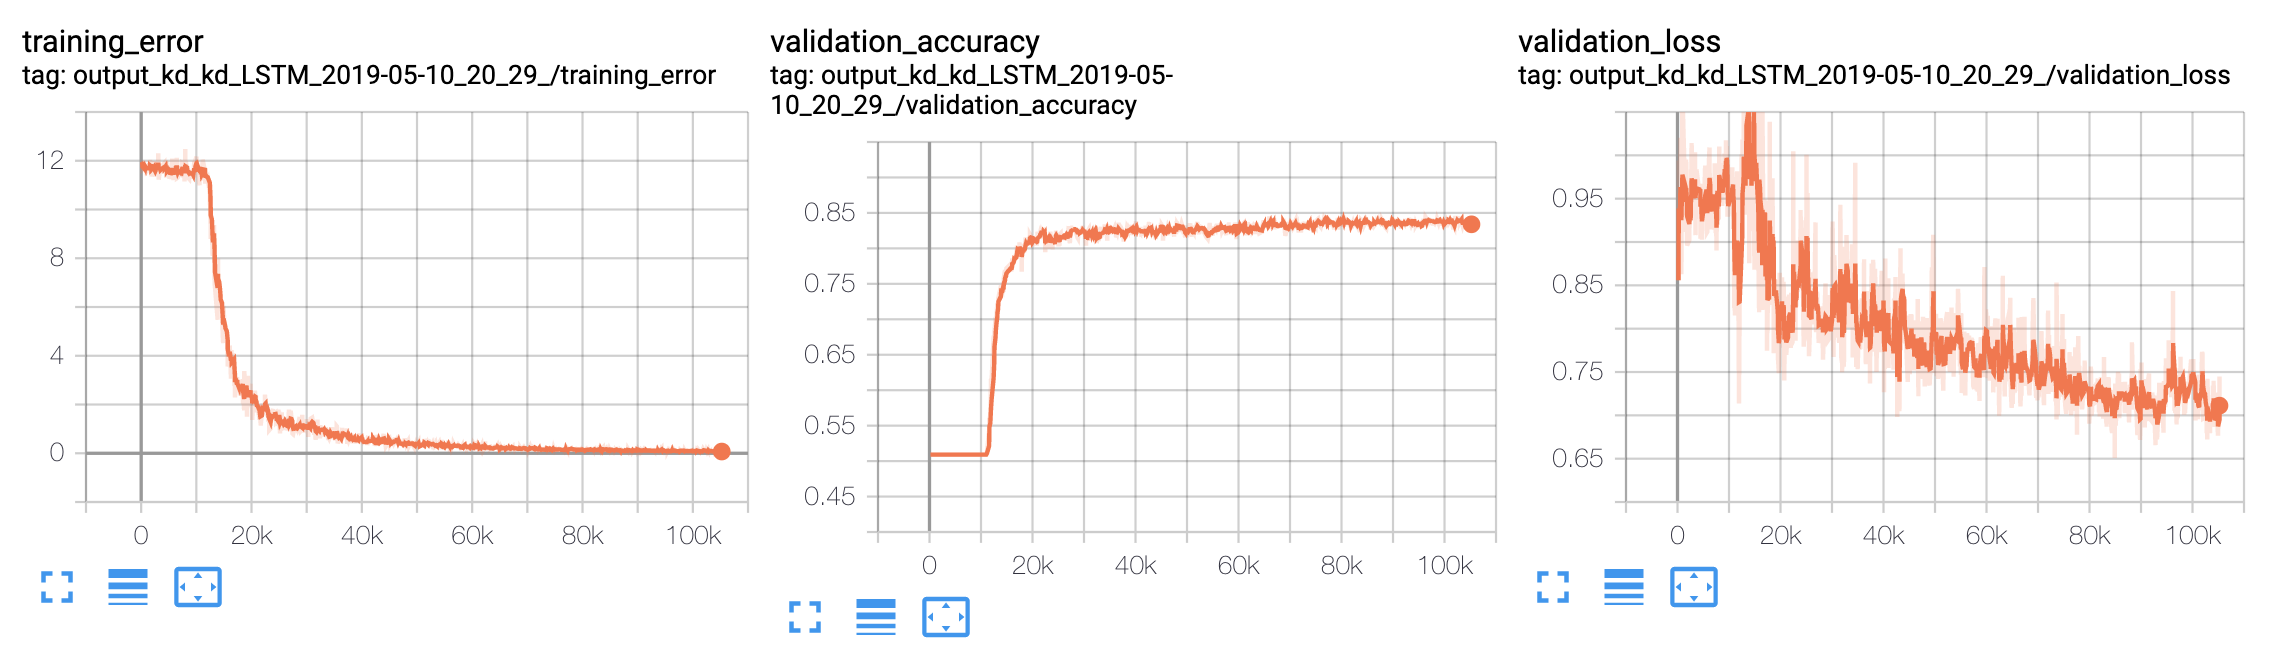
\includegraphics[width=\textwidth]{../figs/kd_lstm_training.png}
\caption{Training loss (left), val. loss (middle), and val. accuracy
(right) plotted against number of batches of training for LSTM KD}
\label{fig:kdlstmloss}
\end{figure*}

Our most striking result is the robust performance of difference pruning. Even
keeping upwards of 99\% of the weights unchanged gives us performance that is
very competitive with the unrestricted model. Most of our experiments are on
SST-2, but we see success with this method on QQP as well, suggesting that
small changes to pretrained BERT are sufficient for performance on a specific
task. 

As expected, difference pruning a higher proportion of the weights decreases
performance, but we are happily surprised at the relatively low magnitude of
this effect even at high prune rates. Pruning with a global threshold rather
than in a stratified way produces distinctly worse results. We suspect this is
due to weights in different layers having different magnitudes, making a global
threshold have an undue effect on layers whose weights tend to be smaller. We
confirm this heterogeneity in \cref{fig:weightsbylayer}.

\begin{figure}[htb]
\centering
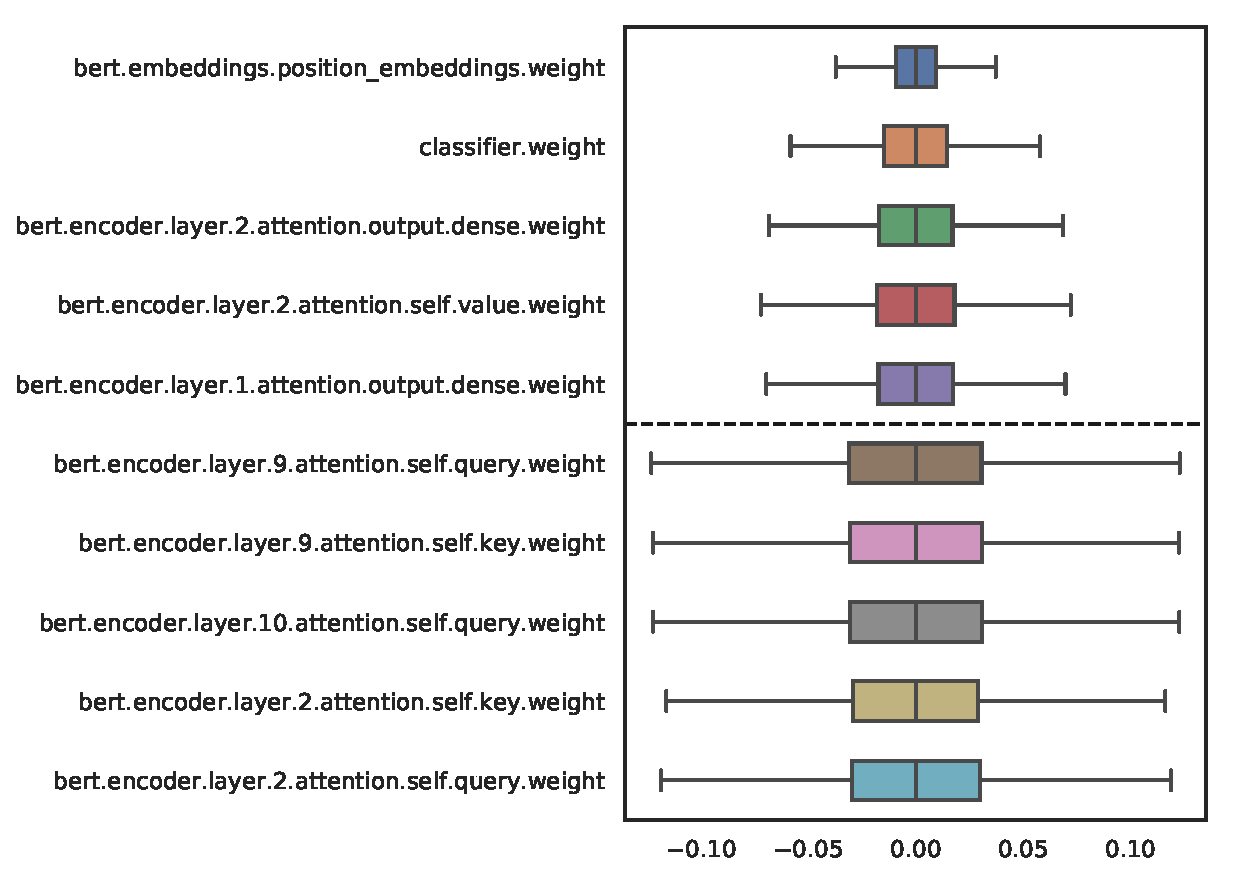
\includegraphics[width=.5\textwidth]{../figs/value_by_layer.pdf}
\caption{Weight distributions for five most/least variable layers}
\label{fig:weightsbylayer}
\end{figure}

Our non-difference distortions are more sensitive to the compression parameter
(whether prune rate or rank reduction rank). We find it difficult to achieve performance
comparable to the uncompressed BERT with a significantly compressed model. Among
the different distortion methods, we favor pruning for its computational
simplicity, and see no evidence that rank reduction achieves better compression.

Remarkably, the fact that pruning and rank reduction incurs significant
losses to the
model seems to show that popular compression techniques that enjoy success
in convolutional neural networks fail to generalize good performance to
transformer-based language networks like BERT. We present some preliminary
evidence in \Cref{fig:singular-values}, where we plot the singular values
in one of the matrices in BERT. The effective rank of the matrix seems
quite high, as the singular values are all sizable, decaying at a rate too
slow for rank reduction techniques to be promising. This suggests that
matrices in BERT are in fact effectively dense, unlike CNNs, where
good compression relies on the effective sparsity of the matrices. 
\begin{figure}[tb]
    \centering
    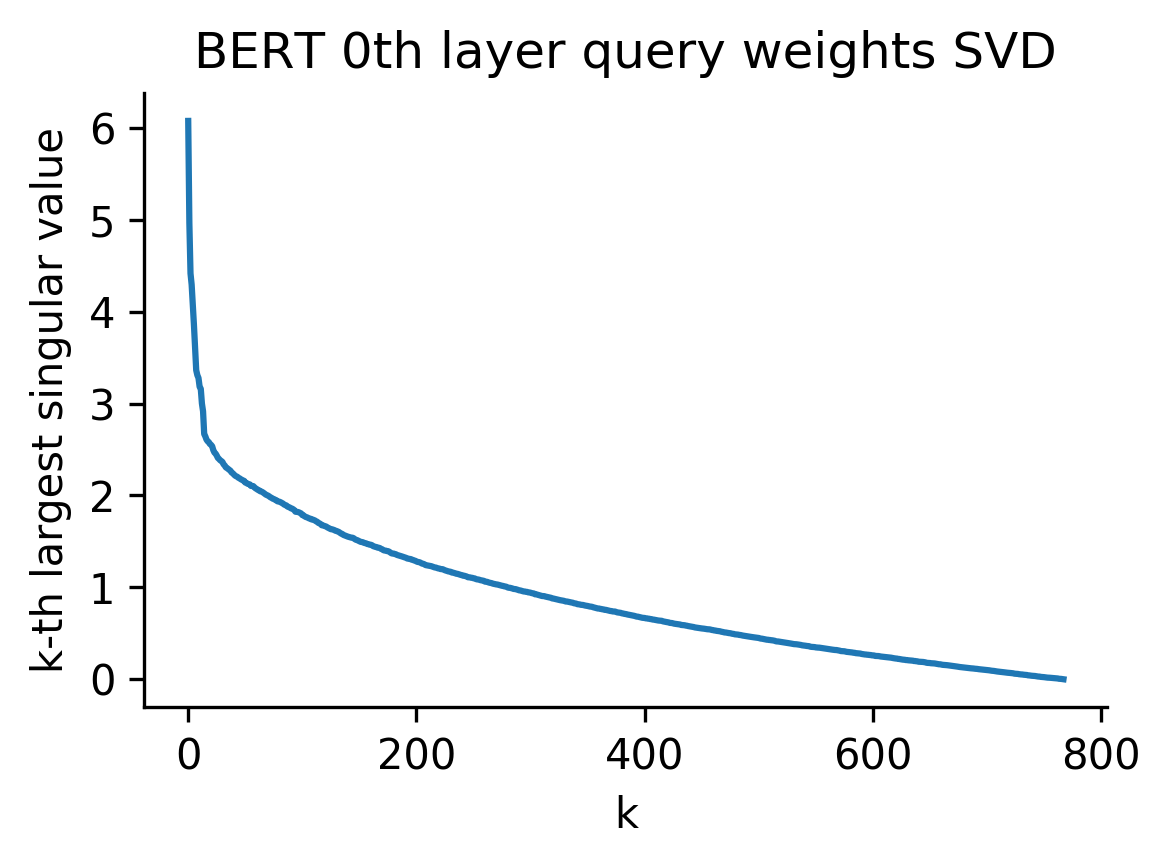
\includegraphics[width=0.5\textwidth]
    {../figs/svd-singular-vals-distribution.png}
    \caption{Distribution of singular values in one of BERT layers}
    \label{fig:singular-values}
\end{figure}

When compared to the performance of a fine-tuned BERT on SST-2, our Knowledge
Distillation results---displayed in \cref{tab:kd_results}---fall short. However,
it is important to note the student networks are also much smaller than BERT. To
isolate the effect of KD, we compare the performance of
\citet{kim2014convolutional}'s CNN trained on the correct labels versus the BERT
probabilities. This suggests a modest performance benefit of two percentage
points in validation accuracy. However, we see no evidence of training being
sped up by using KD.

We also identify some curious behavior in the KD training curves. When training
the LSTM on the BERT outputs, neither training loss nor validation loss decrease
at first. In fact, they stay approximately constant for a couple of epochs. Only
after this prolonged period does loss abruptly start going down, producing a
normal curve from that point forward. We find this---depicted in
\cref{fig:kdlstmloss}---remarkably puzzling. We hypothesize this may be the
effect of our adaptive learning rate starting out too low and taking multiple
epochs to grow to a point where it can meaningfully update parameters. 

\section{Conclusion}

Knowledge Distillation displayed promise by improving student networks'
performance versus training only on the classes $y_i$. However, the student
networks fell short of replicating uncompressed BERT's performance. It is
possible that future variations on our work could achieve competitive
compression. In particular, we restrict our knowledge distillation only to the
samples in the original training set. However, there is no need to perform
training so narrowly since the teacher network can annotate any unsupervised
data. It is likely that doing so would further increase performance, though we
can only speculate as to the magnitude of the benefit.

It is also possible that our choice of student network colored our results. We
aimed for architectures known to work on SST-2 while being much smaller, such as
\citet{kim2014convolutional}'s CNN. It is possible that we aimed too small and
would be better served by a more complex model---possibly even a smaller version
of BERT. Finally, in all our experiments our teacher network is a single
fine-tuned version of BERT. Since teacher network complexity doesn't contribute
to the complexity of the final model, we could instead use an ensemble of BERTs
(or even other models) as our teacher network.

The DeepTwist framework---particularly when combined with difference
pruning---exceeded our expectations for compression. It would be interesting to
test whether this generalizes to a wider array of tasks, particularly since we
only reap compression benefits as we leverage weight sharing over a number of
tasks. Furthermore, from the distortions presented in \citet{lee2018deeptwist},
we did not implement clustering-based quantization because of the significant
computational bottleneck clustering with $k$-means on all of BERT's parameters
posed. Future work could attempt to surmount this obstacle whether through
increased computational resources or a more scalable clustering algorithm.

Finally, we recognize our approaches are but a subset of the ways to go about
compressing large language models such as BERT. Two alternatives stand out as
particularly exciting possible future directions. \citet{liu2019multi} propose a
method for complete weight sharing of BERT's encoder parameters across different
tasks by simultaneously training for all tasks. We believe this approach could
be relaxed through difference pruning to achieve a performance gain relative to
each compression technique in isolation. 

\citet{frankle2018lottery} articulate in their ``lottery ticket hypothesis''
that most networks contain sparse sub-networks which can perform similarly well.
They provide an algorithm for finding these ``lottery tickets'' whose main
differences to DeepTwist are (1) that weights that get distorted to 0 are
permanently masked and kept at 0, and (2) that the algorithm progressively
increases the pruning rate. This framework could serve as a competitive
alternative to DeepTwist, and it would be interesting to see how it performs
with difference pruning.

\section*{Acknowledgements}

We thank Alexander M. Rush and the Harvard CS 287 community, without whom
this work would not have been possible.

\bibliography{paper}
\bibliographystyle{icml2017}

\end{document}
